\documentclass[a4paper, 11pt]{report}
\setcounter{tocdepth}{4}
\setcounter{secnumdepth}{4}
\usepackage{a4}


\usepackage[utf8]{inputenc}
\usepackage{dsfont}
\usepackage{amsmath}
\usepackage{graphicx}
\usepackage{here}
\usepackage[section]{placeins}
\usepackage[ngerman]{babel}
\usepackage{caption}
\usepackage{subcaption}
\usepackage[colorlinks, pdfpagelabels, pdfstartview = FitH, bookmarksopen = true, bookmarksnumbered = true, linkcolor = black, plainpages = false, hypertexnames = false, citecolor = black] {hyperref}
\parindent 0pt


\title{Dokumentation der Projektarbeit}
\author{Florian Weber - 44907}
\date{\today}

\begin{document}
\maketitle	%Deckblatt
\newpage

\tableofcontents 	%Inhaltsverzeichnis
\listoffigures		%Bildverzeichnis
\newpage

\chapter{Vorwort}
Zu Beginn des Projekts war die Carrera Bahn auf dem Stand, dass die Fahrzeuge konventionell sowie automatisiert gesteuert werden konnten. Außerdem war die Rundenzeitmessung und Visualisierung bereits realisiert. Bei der Energieversorgung konnte zwischen Solarstrom und Netzversorgung gewählt werden.
Die Solarstromversorgung wurde pro Bahn durch 2 Solarpanels und einem Tiefsetzsteller mit konstantem Dutycycle hergestellt, die Netzstromversorgung mit einem 15V Schaltnetzteil.

Die Manuelle Steuerung durch den Nutzer wurde realisiert, indem man die klassischen Carrera Drücker, als Variablen Vorwiderstand eingesetzt hat. Im automatisierten Modus musste ein Potentiometer bedient, um die langsame Geschwindigkeit des Autos einzustellen.
In den schnellen Abschnitten der Strecke wurde dieses Poti  durch ein Relais gebrückt und die volle Versorgungsspannung lag an dem Auto an.
\section{Probleme der vorhandenen Carrera Bahn und Zielsetzung zur Projektarbeit}
Der im Vorwort grob erwähnte Aufbau der vorhandenen Anlage wies einige Probleme auf:
\begin{itemize}
	\item 1. Solarstromversorgung und Netzversorgung sind nicht chancengleich ausgeführt.(Die Netzversorgung stellt eine stabilisierte Spannungsquelle dar, die Solarstromversorgung allerdings nicht)
	\item 2. Drift der durch den Poti erzeugten Spannung im automatisierten Modus (Temperaturdrift)
	\item 3. Framerate der Visualisierung ist zu gering, sodass diese immer die selbe Zahlensequenz nach dem Komma anzeigt.
	\item Manchmal wird durch einen Aliasingeffekt das Überschreiten eines Sensors in der Bahn nicht erkannt und die Geschwindigkeit wird nicht umgeschalten.
\end{itemize}
Die oben genannten Probleme sollten durch ein neues Steuer-/Regelkonzept gelöst werden.
\newpage

\chapter{Funktion - Hardware}
	Im Folgenden wird der grundlegende Aufbau der Carrera Bahn erklärt.

	Diese Beschreibung ist immer nur für Bahn-A, da die
	Bahn-B analog dazu funktioniert. Dazu wird immer wieder auf die Abbildung \ref{img:signalfluss}, sowie auf die \\Abbildung
	\ref{img:carrerakomplett} Bezug genommen.
	Die Sensoren in den Schienen teilen die Bahn in 3 Streckenabschnitte auf:
	\begin{itemize}
		\item{1.} Startlinie $\rightarrow$ Vor dem Looping
		\item{2.} Vor dem Looping $\rightarrow$ Nach dem Looping
		\item{3.} Nach dem Looping $\rightarrow$ Startlinie
	\end{itemize}
	Auf Abschnitt 1 und Abschnitt 3 wird im automatisierten Modus die mittlere Geschwindigkeit des Autos geregelt.
	Im Looping (Abschnitt 2) wird die Spannung auf einen konstanten Wert geregelt.
	Die Grenze dafür ist durch die Position der Sensoren festgelegt und somit nicht variabel.
	\begin{figure}[ht]
		\centering
		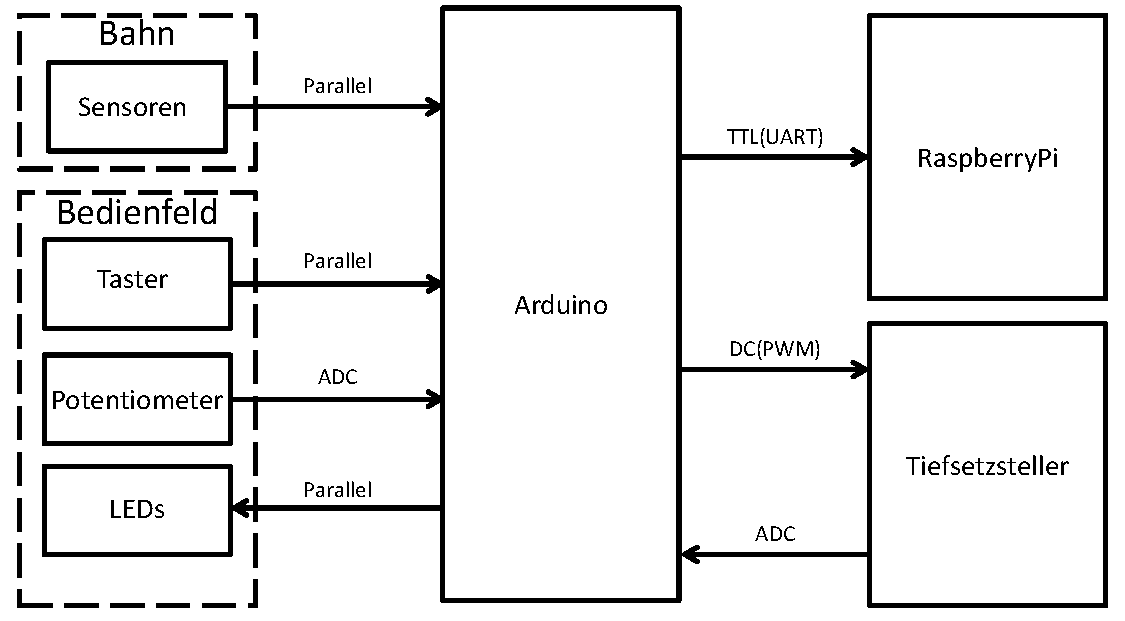
\includegraphics[width=0.85\textwidth]{rec/signalfluss.pdf}
		\caption{Signalfluss}
		\label{img:signalfluss}
	\end{figure}
	\begin{figure}[ht]
	\centering
	\includegraphics[width=0.85\textwidth]{rec/Carrerabahnroh.png}
	\caption{Überblick über die Carrera-Bahn}
	\label{img:carrerakomplett}
	\end{figure}
	\newpage

	\section{Sensoren}
		Pro Schiene gibt es 3 Sensoren die als Gabellichtschranke ausgeführt sind. Sensor 0 befindet sich am Start, Sensor 1 vor dem Looping und 		Sensor 2 Nach dem Looping.\\


		Sensor 0 wird im Wesentlichen nur zur Zeitmessung genutzt.
		Sensor 1 wird genutzt um ein Signal zu generieren, so dass die Steuerung das Auto im Automatik-Modus für den Looping beschleunigen kann.
		Das Signal von Sensor 2 wird schließlich genutzt um nach dem Looping wieder die langsame Geschwindigkeit zu triggern.\\

		Im manuellen Modus dienen die Sensoren nur zur Zeitmessung für die Visualisierung.
		Da die Flanke eines Sensors nur sehr kurz ist, lässt sich diese nicht per Polling ohne Aliasing Effekte digitalisieren. Stattdessen wurden die Hardware	Pin Change Interrupts des Atmega2560 genutzt.
	\section{Bedienschnittstelle}
		\begin{figure}[ht]
			\centering
			\includegraphics[width=0.85\textwidth]{rec/hid.png}
			\caption{Bedienschnittstelle}
			\label{img:hid}
		\end{figure}
		Das HID besteht aus 3 Tastern und einem Wechselschalter mit Mittelstellung je Bahn.
		Der Wechselschalter ist zum Auswählen, ob die Bahn mit Energie aus den Solarpanels betrieben wird, oder mit Netzstrom. Ist Dieser in Mittelstellung, wird die Bahn nicht versorgt und das Auto steht - unabhängig des gewählten Modus.
		Über Taster 0 beziehungsweise Taster 1 lässt sich der Modus der Bahn auswählen, welcher durch die LEDs bei den Tastern signalisiert wird. \\Hier steht Automatik und Manuell zur Auswahl.
		Mit Taster 2 lässt sich der Regler der Bahngeschwindigkeit genauer -  Spannung außerhalb des Loopings, auf seinen Startwert zurücksetzen.
	\section{Arduino}
		Beim Arduino handelt es sich um einen einfachen Arduino Mega 2560 ADK.\\
		Dieser wurde gewählt da es sich um eine preiswerte Platine handelt, die bereits die wichtigsten Beschaltungen des Mikrocontroller enthält wie zum beispiel die Abblockcondensatoren an der Versorgungsspannung aber auch einen USB-Seriell Wandler den man nutzen kann um sich Daten parallel zum Prozess an ein Terminal auszugeben.
		Letzteres lässt sich sehr gut für das Debugging nutzen.
	\section{RaspberryPi}
		Die Visualisierung ist durch ein RaspberryPi Model 3 B realisiert. Dieser empfängt per Uart die codierten Signale der Sensoren, sowie des Reset Tasters der Visualisierung.
		Die Visualisierung war zu Beginn der Projektarbeit bereits vorhanden und in Form eines Python Skripts implementiert.
	\section{Tiefsetzsteller}
		Die Tiefsetzsteller fungieren als Stellglieder der Spannungsregelungen der Bahnen.
		Jeder bekommt sein PWM-Signal(Steuergröße) direkt vom Arduino. Desweiteren ist über ein Shunt eine
		Strommessung realisiert. Der Wert liegt zwar im Arduino digital vor, wird allerdings nicht weiter
		verarbeitet und ist lediglich für weiterführende Projekte gedacht. Da die Ausgangsspannung des
		Tiefsetzstellers größer sein kann wie die Referenzspannung des ADC,
		wird diese über einen Spannungsteiler angepasst und auf einen Kanal des ADC geführt.
		Diese Spannung stellt die Regelgröße dar.
	\newpage

\chapter{Software}
	\section{RaspberryPi}

		Bei der Software die auf dem RaspberryPi ausgeführt wird, handelt es sich um ein Python Skript.
		Dieses war zu Beginn der Projektarbeit bereits vorhanden und hat die Sensoren
		der Bahn parallel eingelesen. Mit den Flanken der Sensoren wurde die Rundenzeit gemessen
		und die Bestzeit ermittelt.\\
		Dieses Skript wurde größtenteils übernommen und lediglich in der Richtung abgeändert,
		dass die Trigger-Signale der Sensoren nun über die Serielle Schnittstelle dem Pi mitgeteilt wurden.
		Desweiteren wurden diverse Bugs behoben wie zB die zu geringe Framerate der Visualisierung.
		Als serielle Schnittstelle wurde "ttyAMA0" benutzt.
		\newpage
	\section{Arduino}
		Die Software des Arduinos wurde, wie oben bereits erwähnt, nicht in der Arduino Entwicklungsumgebung
		geschrieben. Stattdessen habe ich auf die IDE "AtmelStudio 7" zurückgegriffen und den Mikrocontroller
		per ISP beschrieben. Der Bootloader des Arduino musste dazu entfernt werden.
		Gründe dazu waren unter anderem die Wahl der Sprache C++,
		aber auf die Möglichkeit direkt auf die Hardware zuzugreifen(Timer, Hardwareinterrupts...).
		Letzteres ist notwendig um das Timing des Controllers exakt zu steuern.\\
		\subsection{Interrupts}
		\begin{figure}[ht]
			\centering
			\begin{subfigure}{0.47\textwidth}
				\centering
				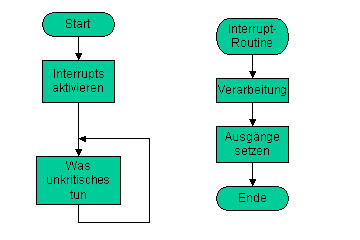
\includegraphics[width=1.1\textwidth]{rec/Interrupt_Programme.png}
				\caption{Interruptgesteuerter \\Programmablauf}
				\label{InterruptgesteuerterProgrammablauf}
			\end{subfigure}
			\begin{subfigure}{0.47\textwidth}
				\centering
				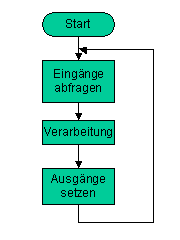
\includegraphics[width=0.55\textwidth]{rec/Sequentielle_Programme.png}
				\caption{Sequentieller \\Programmablauf}
				\label{SequentiellerProgrammablauf}
			\end{subfigure}
			\caption[Möglichkeiten zum Programmablauf]{Möglichkeiten zum Programmablauf
			\\Quelle:Mikrocontroller.net}
			\label{Programmablauf}
		\end{figure}
Der Programmablauf ist größtenteils Interruptgesteuert.
			Dies hat den Vorteil, dass das Timing nichtmehr von der Länge der MainLoop abhängt und Dinge wie zum  Beispiel der Regelagorythmus immer in der selben Frequenz ausgeführt werden.
			Interruptquellen des Programms sind:
			\begin{itemize}
				\item Timer  (Abschnitt \ref{subsubsec:Timer})
				\begin{itemize}
					\item[1.] Timer1, Compareregister B match
					\item[2.] Timer3, Compareregister A match
					\item[3.] Timer4, Compareregister A match
				\end{itemize}
				\item Pin Change Interrupts (Abschnitt \ref{subsubsec:PCINT})
				\begin{itemize}
					\item[4.] PCINT0\underline{ }vect
					\item[5.] PCINT1\underline{ }vect
					\item[6.] PCINT2\underline{ }vect
				\end{itemize}
				\item Analog Digital Converter
				\begin{itemize}
					\item[7.] ADC\underline{ }vect  (Abschnitt \ref{subsubsec:ADCINT})
				\end{itemize}

			\end{itemize}
			\newpage
			Zu Anfang des Programms wird die ganze Peripherie initialisiert, und die Variablen mit ihren default Werten geladen.
			Anschliesend werden die Interrupts global freigegeben. Ab hier ist die Steuerung funktionsfähig.
			\subsubsection{Timer}\label{subsubsec:Timer}
			Für Die Funktion der Steuerung werden viele Timer benötigt.\\
			Da im Mikrocontroller allerdings nur begrenzt Timer zur Verfügung stehen, wurde deren Funktionalität in einem Software-Timer nachgebildet.
			Dieser erhält sein Takt von einem Hardwaretimer.
			Die Verwendung der Hard- sowie Softwaretimer kann der Tabelle \ref{tab:belegungTimer} entnommen werden.
				\begin{table}[ht]
					\begin{tabular}{|l|l|l|}
						\hline
						\textbf{Timer} & \textbf{Funktion}\\
						\hline
						\hline
						 & \\
						Hardwaretimer &\\
						\hline
						\hline
						Timer0 & Generierung der 2 PWM Kanäle für die Tiefsetzsteller\\
						\hline
						Timer1 & Auslösen der Analog Digital Wandlung\\
						\hline
						Timer2 & Ohne Verwendung\\
						\hline
						Timer3 & Trigger für Spannungsregelung\\
						\hline
						Timer4 & Trigger für Softwaretimer\\
						\hline
						\hline
						 & \\
						Softwaretimer &\\
						\hline
						\hline
						0..1 & Zeitmessung Abschnitt 3 (Nach dem Looping $\rightarrow$ Startlinie)\\
						\hline
						2..7 & Entprellen der Bahnsensoren\\
						\hline
						8..14 & Entprellen der HID Taster\\
						\hline
						15..16 & Ohne Verwendung\\
						\hline
						17 & Trigger für Zeitmessung Resettaster\\
						\hline
					\end{tabular}
					\caption{Belegung der Hard- sowie Softwaretimer}
					\label{tab:belegungTimer}
				\end{table}
			\subsubsection {Pin Change Interrupt}\label{subsubsec:PCINT}
			Wenn ein Auto nun auf, Beispielsweise Sensor 0 (Bahn A, am Start), fährt wird der Pegel kurze Zeit \emph{low} und nach verlassen des Sensors wieder \emph{high}.\\ Da Sensor 0 an PCINT16 angeschlossen ist und 16 im Bereich [16,23] liegt, wird das letzte Pin Change Interrupt, PCINT2\underline{ }vect, zweimal ausgelöst. In der ISR (Interrupt Service Routine) muss nun unterschieden werden, durch welchen Pin das Interrupt ausgelöst wurde.
			Außerdem gibt es die zwei Möglichkeiten:
				\begin{itemize}
					\item war es ein High $\rightarrow$ Low Übergang
					\item war es ein Low $\rightarrow$ High Übergang
				\end{itemize}

			Zum Entprellen des Eingangs wird direkt, nachdem das Event gehandelt wurde, der Eingang deaktiviert. Danach wird ein Software-Timer gestartet der den Eingang nach dessen Ablauf wieder aktiviert. Mit diesem einfachen Prinzip wird sichergestellt, dass wenn das Auto beim Überahren des Sensors das dementsprechende Event nur einmal triggert.
			Analog zu diesem Sensor 0, ist dies für jeden Sensor sowie Taster realisiert. Die Belegung der benutzten Pin Change Interrupts kann Tabelle \ref{tab:belegungpcint} entnommen werden.
			\begin{table}[ht]
				\begin{tabular}{|l|l|l|}
					\hline
					Zugehörigkeit & Signal & Bezeichnung\\
					\hline
					\hline
					PCINT0\underline{ }vect & PCINT4 & Button: B-Automatik\\
					\hline
											& PCINT5 & Button: B-Manuell\\
					\hline
											& PCINT6 & Button: A-Automatik\\
					\hline
					\hline
					PCINT1\underline{ }vect & PCINT9 & Button: A-Reset\\
					\hline
											& PCINT10 & Button: B-Reset\\
					\hline
					\hline
					PCINT2\underline{ }vect & PCINT16 & Sensor: 0\\
					\hline
											& PCINT17 & Sensor: 1\\
					\hline
											& PCINT18 & Sensor: 2\\
					\hline
											& PCINT19 & Sensor: 3\\
					\hline
											& PCINT20 & Sensor: 4\\
					\hline
											& PCINT21 & Sensor: 5\\
					\hline
											& PCINT22 & Button: Reset/Shutdown Pi\\
					\hline
											& PCINT23 & Button: A-Manuell\\
					\hline
				\end{tabular}
				\caption{Belegung der Pin Change Interrupts}
				\label{tab:belegungpcint}
			\end{table}
			\subsubsection{Analog Digital Converter Interrupt}\label{subsubsec:ADCINT}
			zum Betrieb des Zustandsautomats welcher den Multiplexer des ADC steuert ist ein Interrupt notwendig, welches ausgelöst wird, wenn der ADC eine MEssung abgeschlossen hat. Dieser Automat is genauer in Abschnitt \ref{subsec:ADC} beschrieben.

			%erklärung an diesem
	\subsection{Regler}
		\begin{figure}[ht]
			\centering
			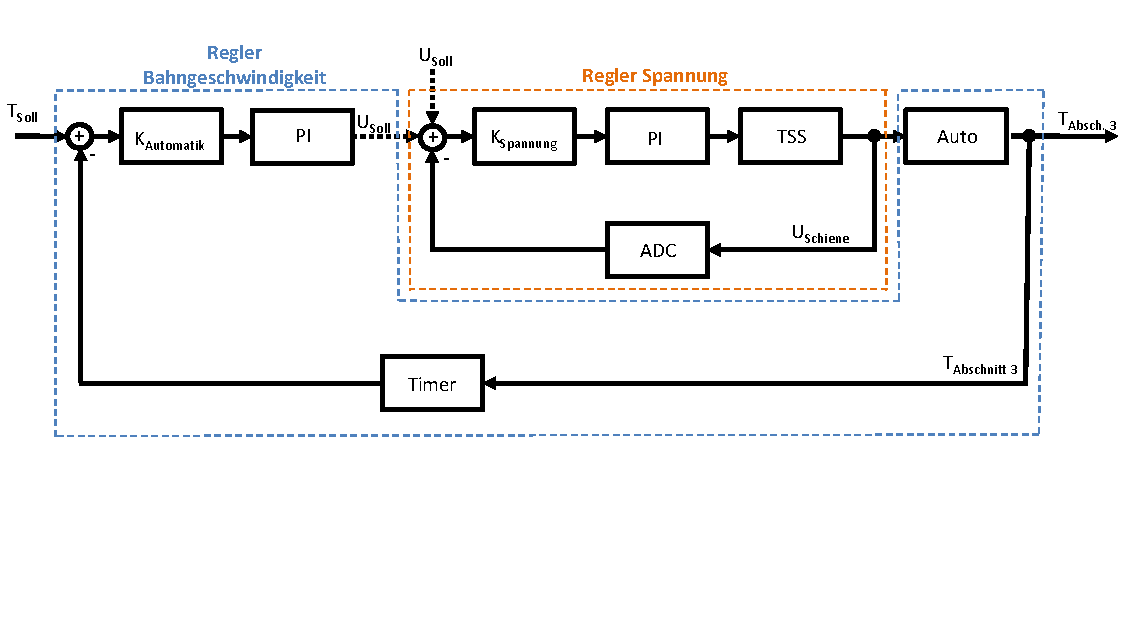
\includegraphics[width=\textwidth]{rec/Regler.pdf}
			\caption{Kaskadenreglung Bahngeschwindigkeit}
			\label{img:Regelung}
		\end{figure}
		Die Regelung für die Bahngeschwindigkeit ist als Kaskadenregelung (Abbildung \ref{img:Regelung}) ausgeführt.
		Dem Führungsregler wird eine Sollzeit für Streckenabschnitt 3 vorgegeben, dieser gibt nun die Sollspannung für den Folgeregler vor.
		Der Folgeregler hat als Stellgröße den Duty-Cycle des zugehörigen Tiefsetzstellers und regelt die Spannung auf der Schiene auf den gegebenen Wert.
		Der Regelalgorithmus des Spannungsreglers wird in festen Zeitabständen, vorgegeben durch OCR3 (Overflow Compare Register Timer3), zyklisch aufgerufen.
		Der Regelalgorithmus des Reglers der Bahngeschwindigkeit wird immer dann aufgerufen, wenn ein neuer Zeitwert für den Streckenabschnitt 3 vorliegt.
		Dieses Vorgehen ist sehr störanfällig, allerdings ist es die einzige Möglichkeit, einen solche Regelung mit den vorhandenen Sensoren zu realisieren. \\
		Der Vorfaktor des Führungsreglers ist eher verhältnismäßig klein gewählt, um ein Überschwingen möglichst zu verhindern.
		Die gerade beschriebene Regelstrategie ist als solche nur im Automatik-Modus aktiv.\\
		Im manuellen Modus wird die Sollspannung direkt durch den Handregler vorgegeben.
		\newpage
	\subsection{Analog Digital Wandler}\label{subsec:ADC}

		Der Mikrocontroller des Arduinos (Atmel Atmega 2560) hat bereits einen 10 bit ADC (Analog Digital Converter) auf dem Chip integriert, dass auf einen externen Wandler verzichtet werden kann.
		Da der Wandler immer nur einen Messung durchführen kann, hat der Hersteller ein (MUX) Multiplexer integriert um zwischen den einzelnen ADC Pins des Mikrocontroller durchzuschalten.
		Die Belegung der ADC Pins des Mikrocontrollers ist in Tabelle \ref{tab:AnhangBelegungArduino} enthalten.

		Wenn die angestoßene Messung des ADC abgeschlossen ist, wird ein Interrupt ausgelöst.


		Die Steuerung des Multiplexers erfolgt über ein Zustandsautomat der immer dann getriggert wird, wenn wenn die letzte Messung des ADC abgeschlossen ist.

		\begin{figure}[ht]
			\centering
			\includegraphics[width=0.3\textwidth]{rec/ADCAutomat.png}
			\caption{Zustandsautomat Analog Digital Converter Kanal}
			\label{img:ADCMUX}
		\end{figure}

\subsection{PWM Generierung Tiefsetzsteller}
\begin{figure}[th]
	\centering
	\begin{subfigure}{0.34\textwidth}
		\centering
		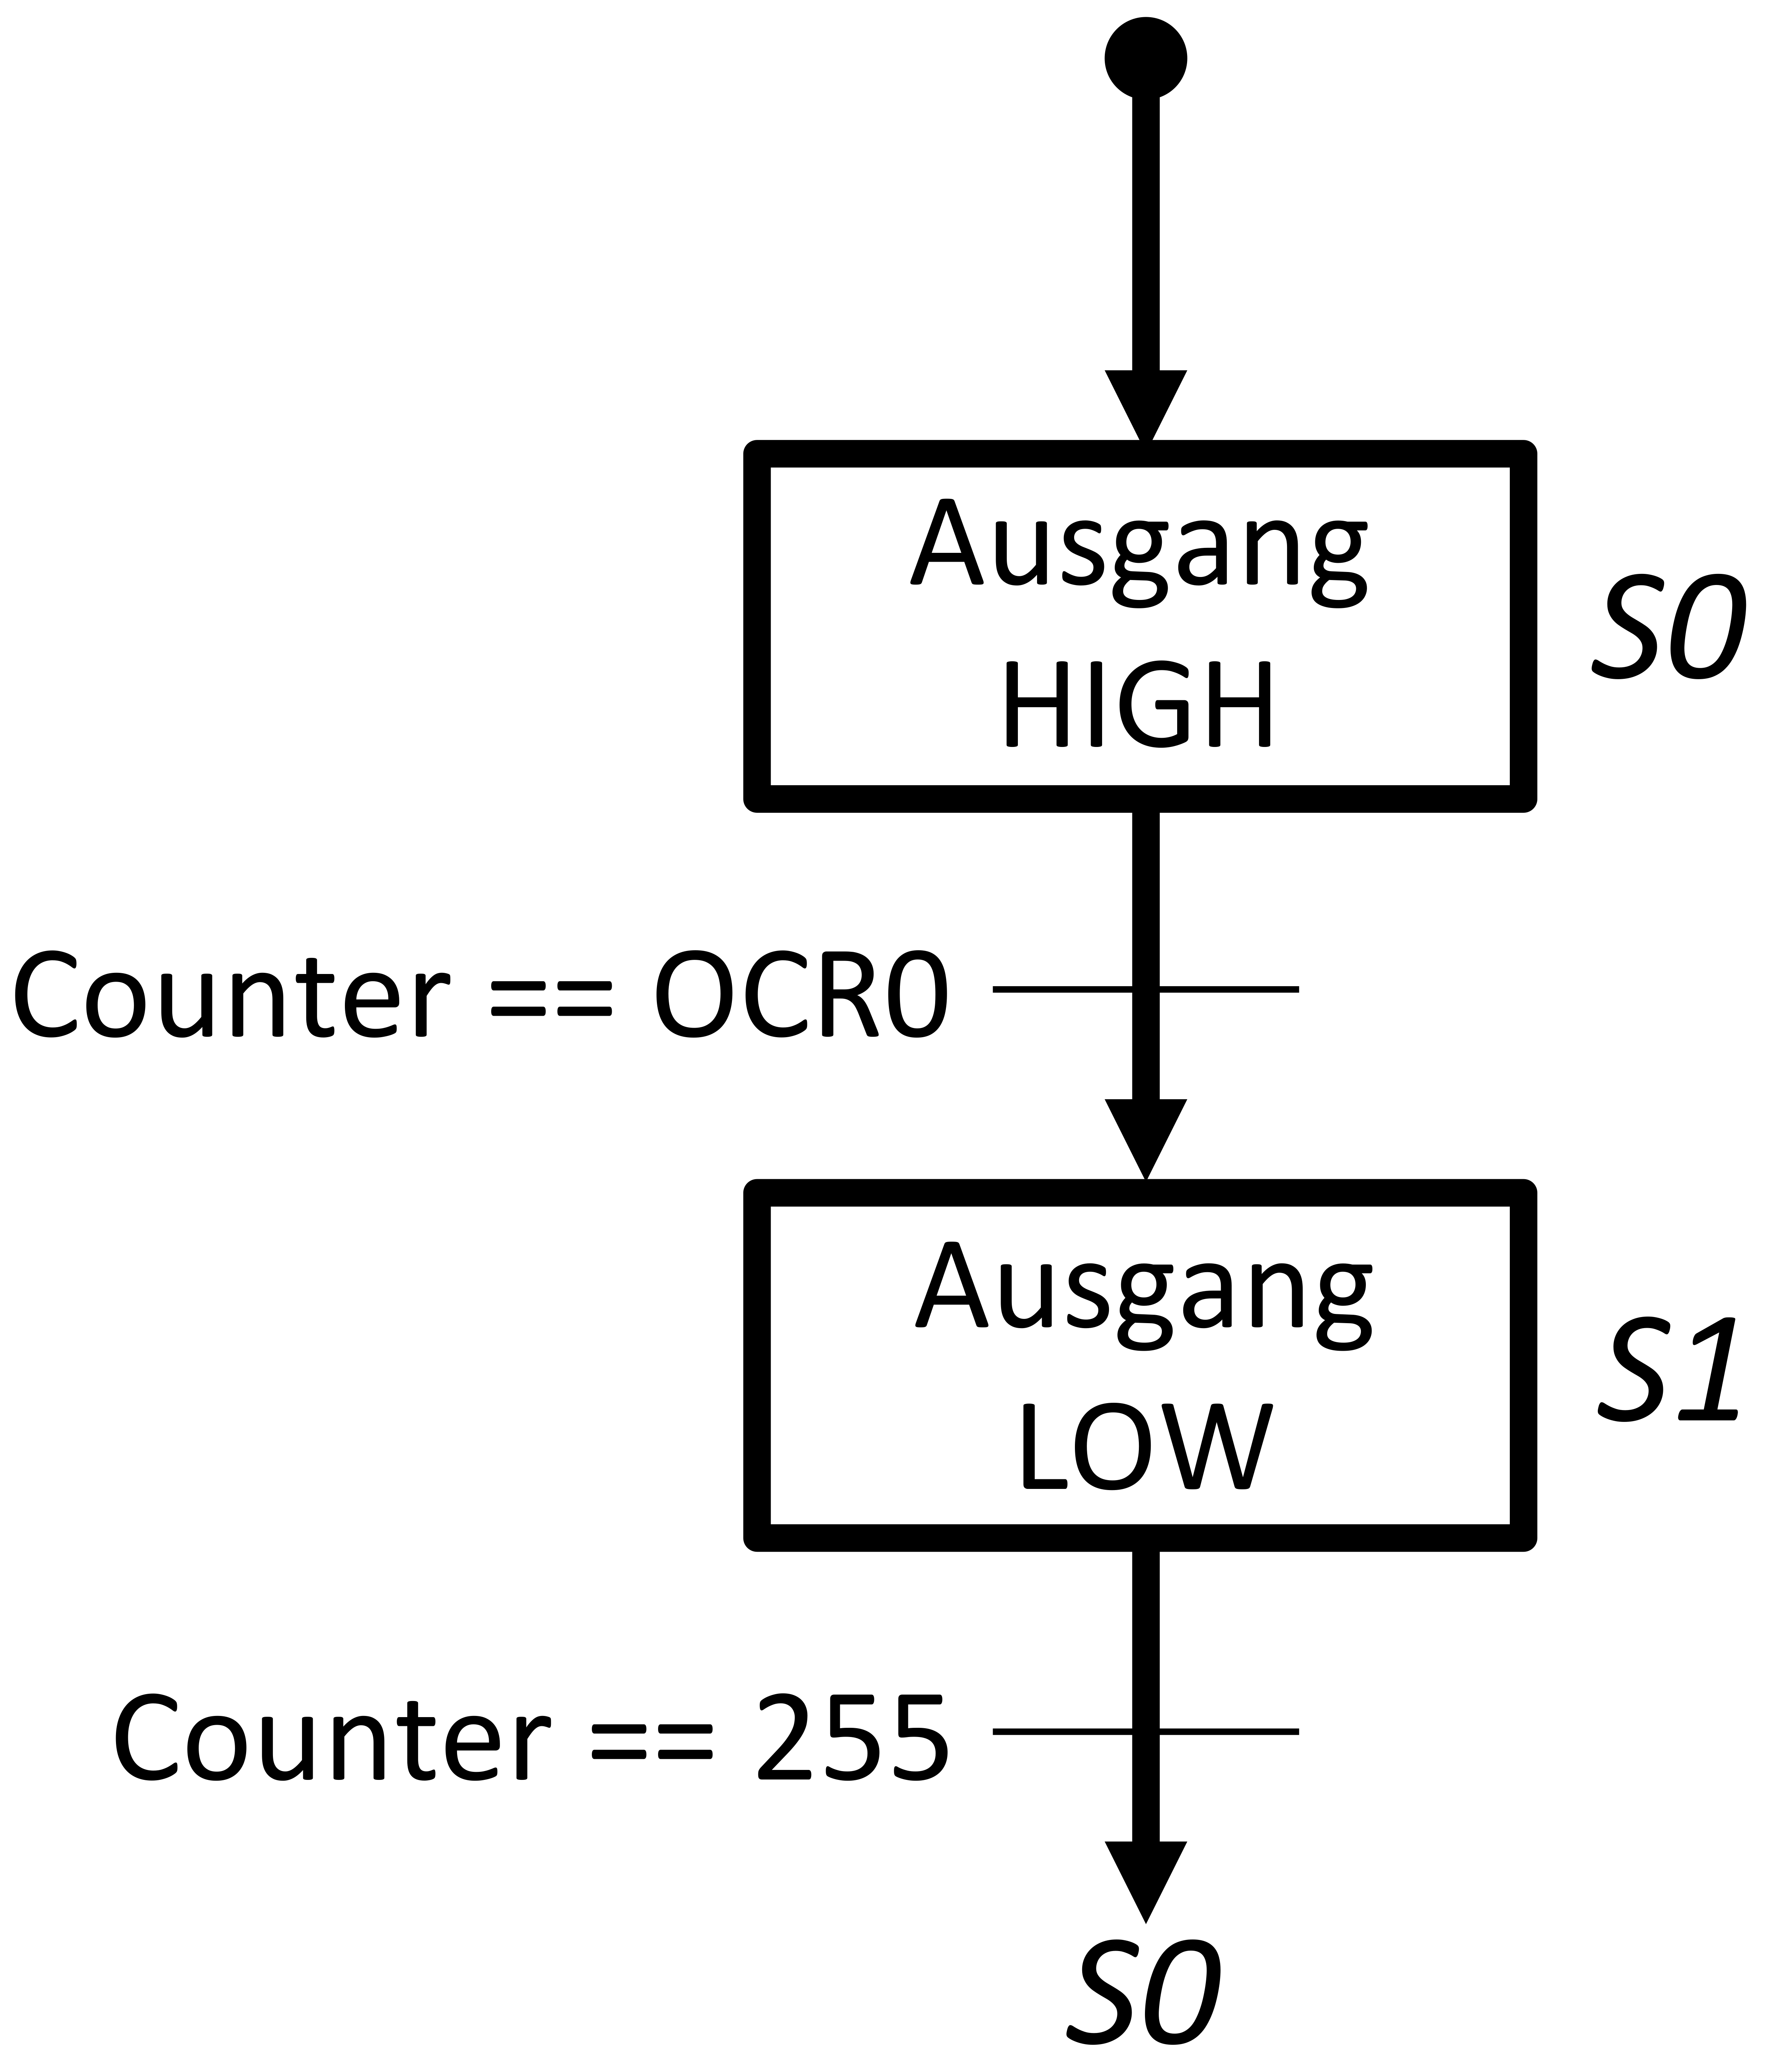
\includegraphics[width=0.95\textwidth]{rec/zustandsautomatPWM.png}
		\caption{Zustandsautomat PWM Generierung}

	\end{subfigure}
	\begin{subfigure}{0.64\textwidth}
		\centering
		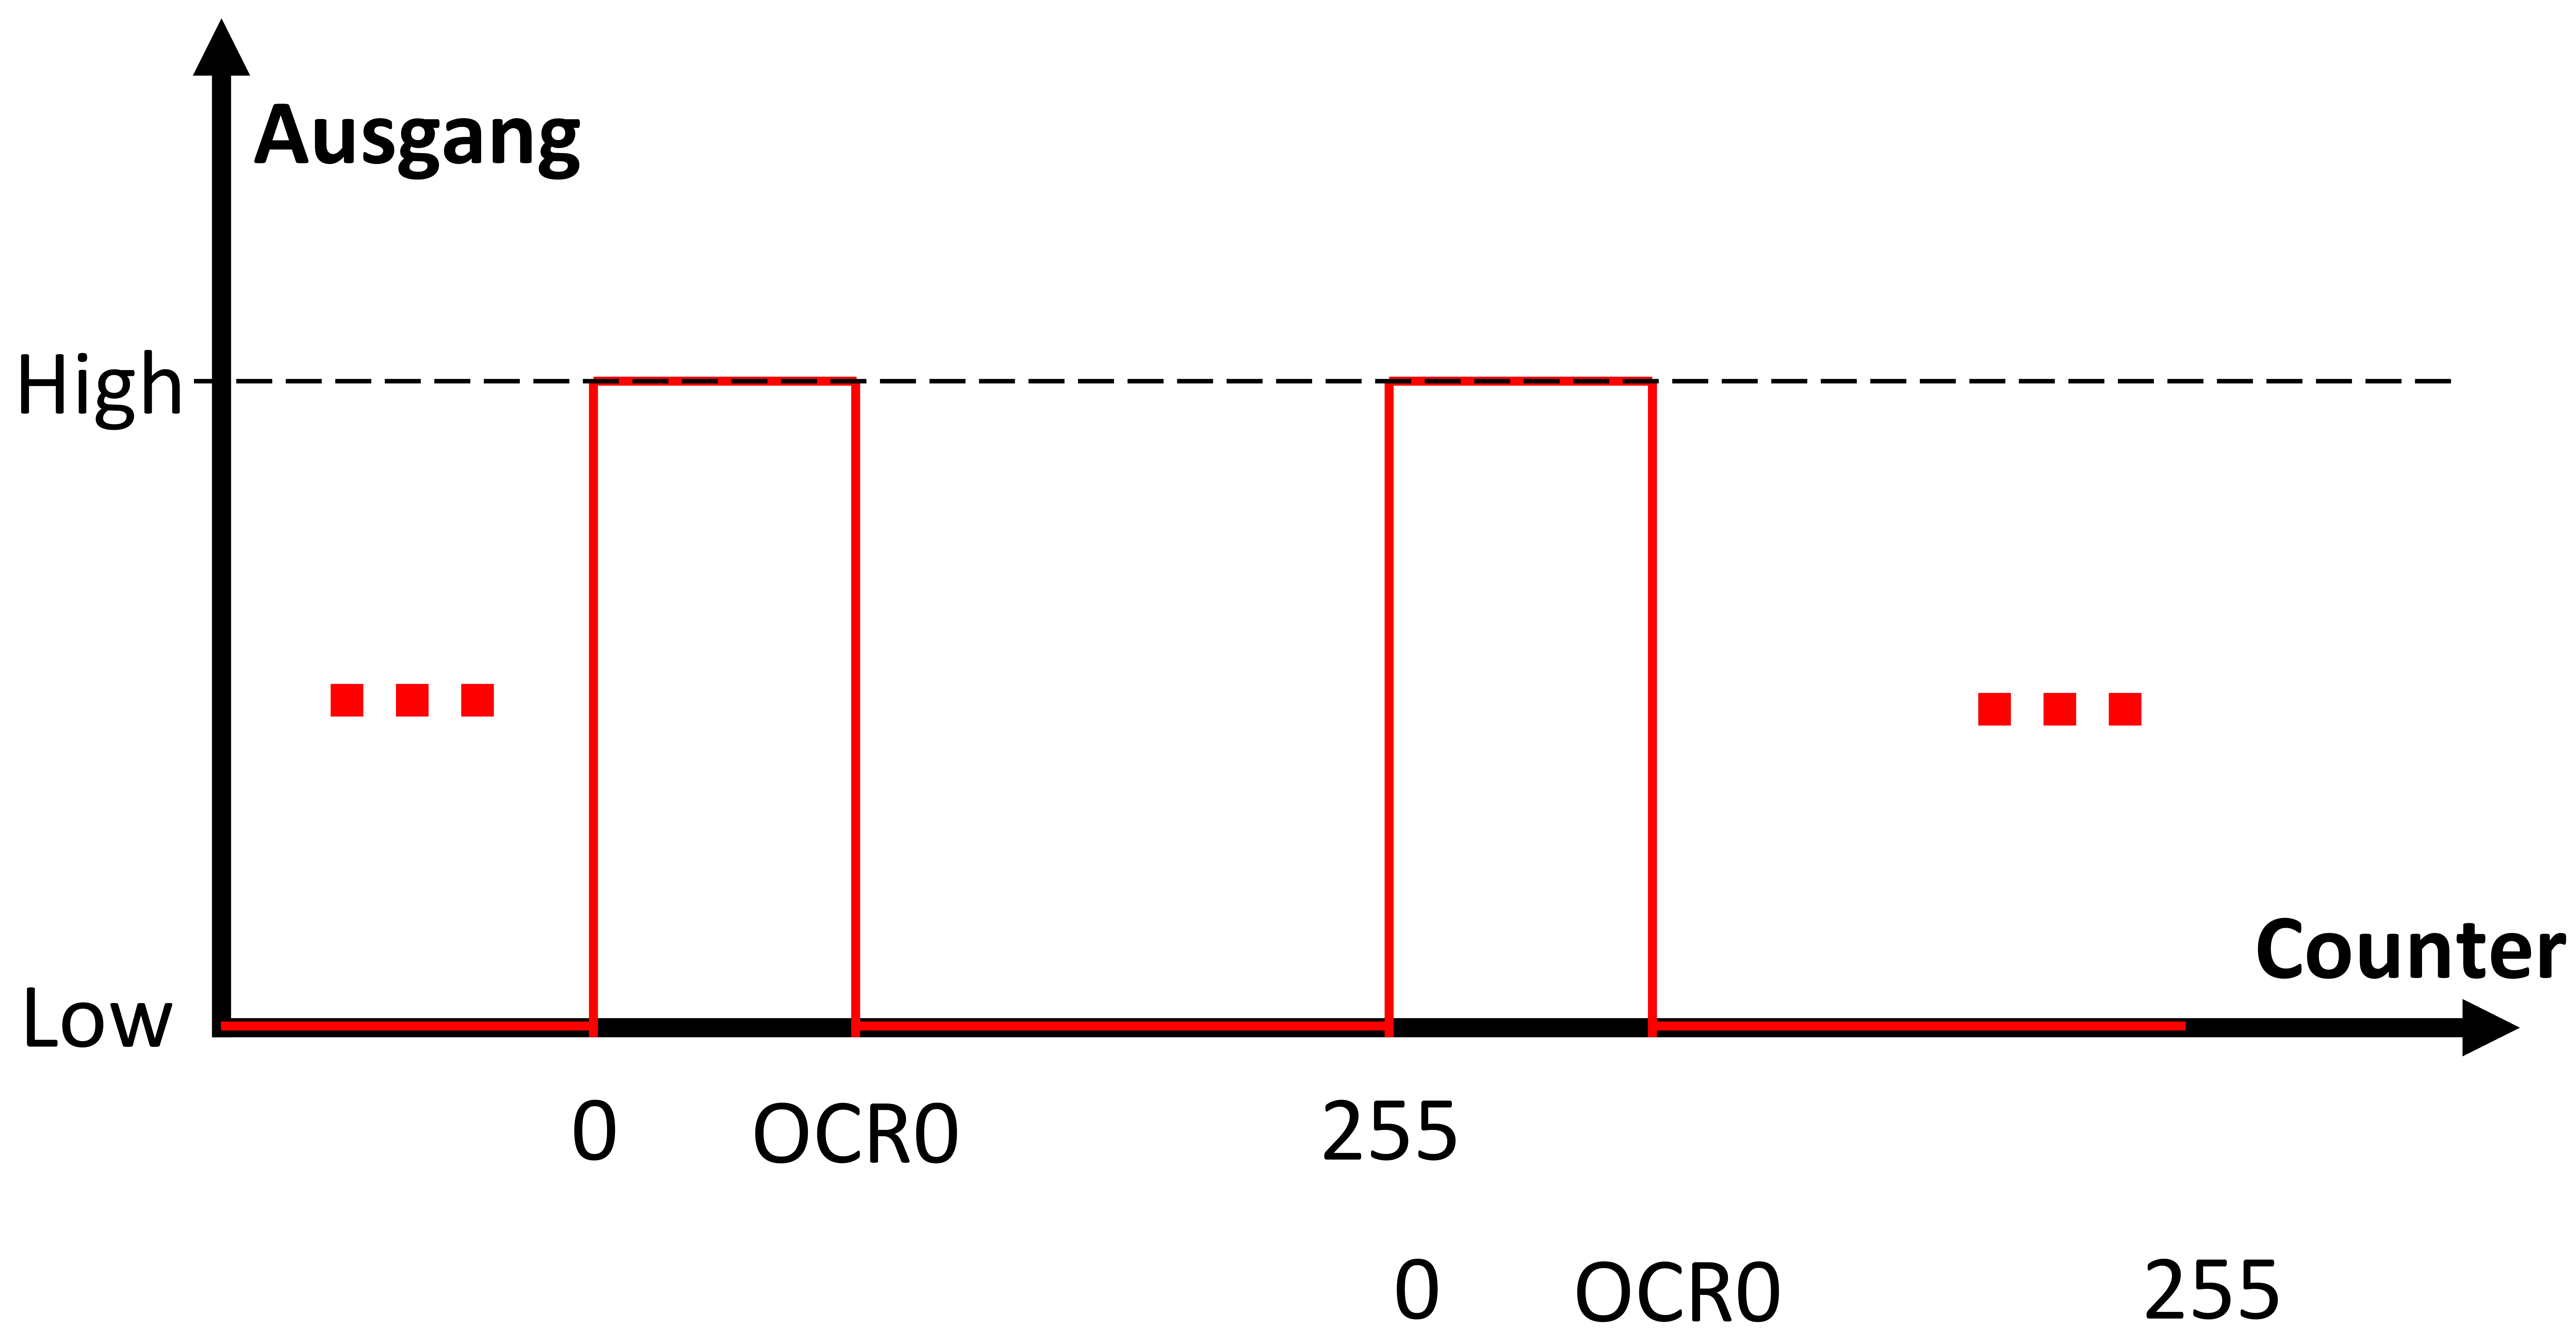
\includegraphics[width=0.95\textwidth]{rec/graphPWM.png}
		\caption{Ausgang PWM-Pin als Funktion des Zählerstands}

	\end{subfigure}
	\label{fig:PWMGEN}

\end{figure}

%wie wird pwm generiert

\chapter{Bedienungsanleitung}
\section{Einschalten}
	Die Anlage muss zum einschalten lediglich mit der Netzversorgung verbunden werden. Sobald Die Anlage Spannung hat, bootet der RaspberryPi selbständig und startet die Visualisierung. Ab diesem Punkt ist Die Carrerabahn betriebsbereit und im Modus Manuelles Fahren (Abschnitt \ref{subsec:ManuellesFahren}).
\section{Betrieb}
	\begin{figure}[ht]
		\centering
		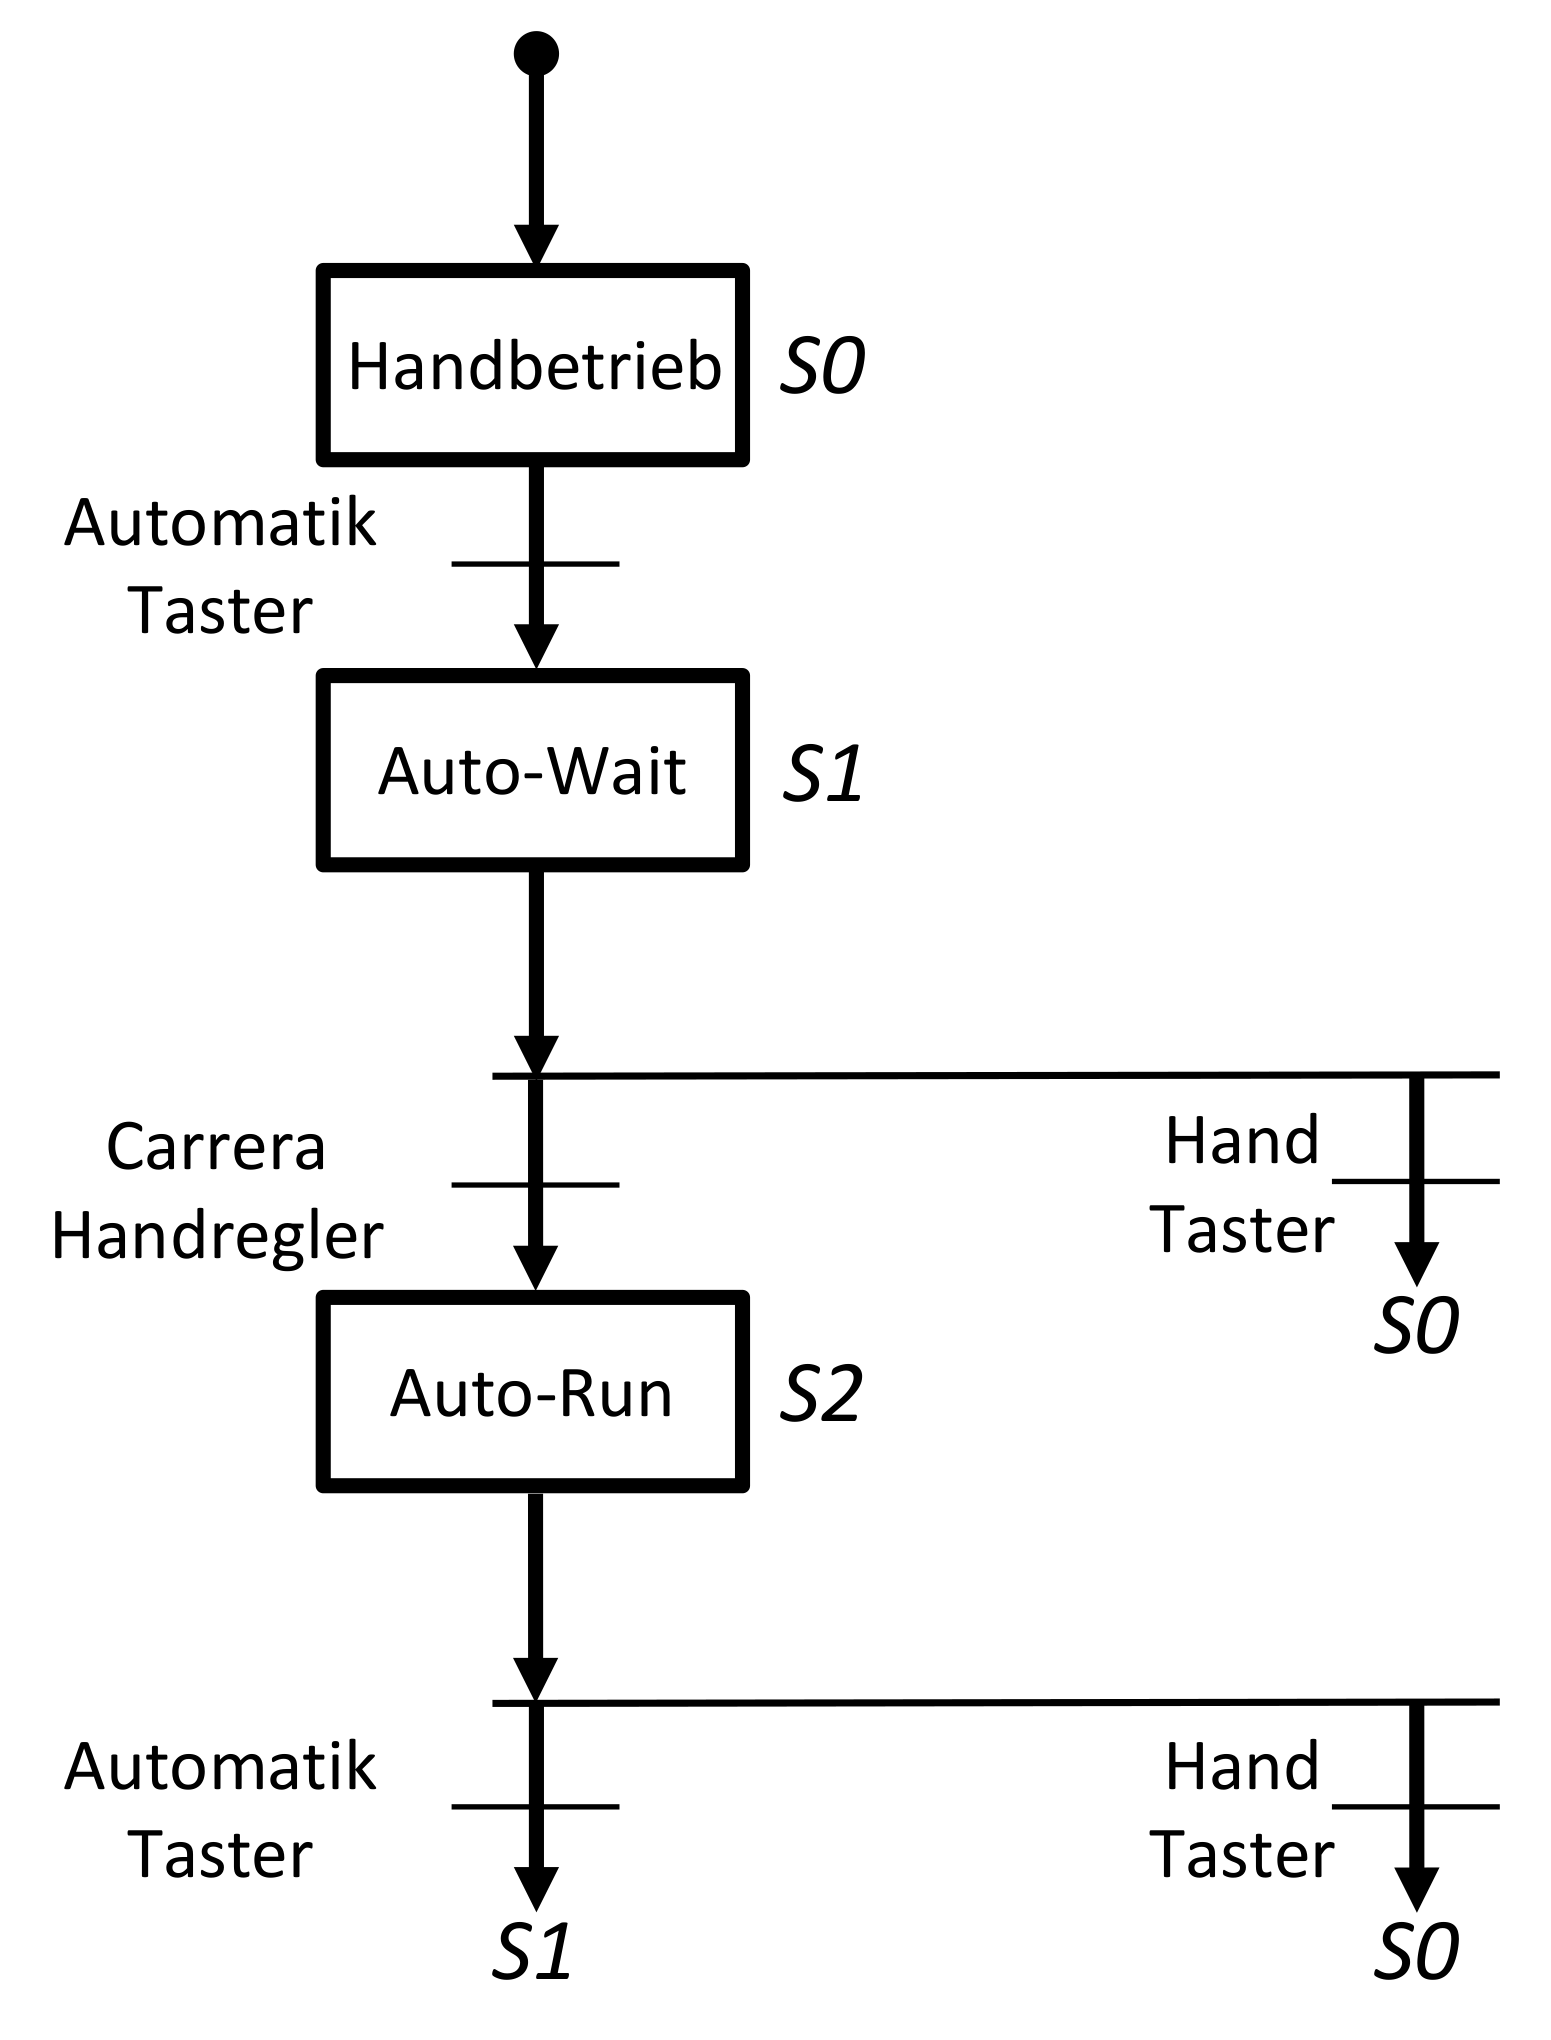
\includegraphics[width=0.5\textwidth]{rec/modiAuswahl.png}
		\caption{Zustandsautomat Betriebsmodi}
		\label{img:Betriebsmodi}
	\end{figure}
	Die Carrera-Bahn beherrscht 2 Modi.
	\begin{itemize}
		\item Manuelles Fahren
		\item Automatisiertes Fahren
	\end{itemize}
	Die Modi können unabhängig voneinander auf beiden Bahnen gewählt werden, sodass man zum Beispiel manuell gegen ein automatisiertes Fahrzeug antreten kann. Die Wahl eines dementsprechenden Modus wird durch eine Led über, beziehungsweise unter, des jeweiligen Tasters des gewählten Modus signalisiert. Außerdem kann die Energieversorgung jeder Bahn mit dem entsprechenden Wechselschalter ausgewählt werden. Unabhängig des gewählten Modus, wird in der Visualisierung die Zeit der 2 Abschnitte, sowie die Rundenzeit angezeigt. Nach 30 Runden ist das Rennen vorbei und die Visualisierung wird statisch.
	Der Wechsel zwischen den Modi findet nach Abbildung \ref{img:Betriebsmodi} statt und ist in den jeweiligen Abschnitten genauer erklärt.
	\subsection{Manuelles Fahren}\label{subsec:ManuellesFahren}
		Im Modus Manuelles Fahren kann das Fahrzeug konventionell über die orginalen Carrera Handregler gesteuert
		werden.
	\subsection{Automatisiertes Fahren}
		Der Automatisierte Modus ist aufgeschlüsselt in 2 Zustände:
		\begin{itemize}
			\item Auto-wait
			\item Auto-run
		\end{itemize}
		\subsubsection{Auto-Wait}
		Immer wenn in den Modus des Automatisierten Fahrens gewechselt wird, startet die Steuerung in
		Auto-wait und das Auto steht.
		Durch kurzes durchdrücken des zugehörigen Handreglers wechselt das Auto in den Auto-run Zustand.
		\subsubsection{Auto-Run}
			Im Auto-run Zustand fährt das Auto selbständig. Durch die Regelung der mittleren Geschwindigkeit des langsamen Streckenabschnitts braucht das Auto einige Runden um die optimale Spannung für diese Geschwindigkeit zu finden.

			In der Visualisierung ist die Strecke von der Startlinie bis vor den Looping in Streckenabschnitt 1 zusammengefasst.
			Der Rest einer Runde (vor dem Looping bis zur Startlinie) bildet Streckenabschnitt 2.
\section{Ausschalten}
Um die Anlage ordnungsgemäß herunterzufahren, muss man den Reset Taster am HMI (Abbildung \ref{img:hid} - Reset Visualisierung) mindestens 5 Sekunden gedrückt halten.
Nun muss man warten bis der RaspberryPi komplett heruntergefahren ist. Dies ist daran zu erkennen dass die grüne Led auf dem RaspberryPi nichtmehr blinkt und der Bildschirm in den Standby-Modus schaltet.
\chapter{Zusammenfassung}

%verbesserung:
	%pi auch Solarstrom
	%Looping bürsten kontakt


\chapter{Anhang}
\section{Pinbelegung}

\begin{table}
		\begin{tabular}{|l|l|}
			\hline
			\textbf{Sub-D Pin} &\textbf{Funktion}\\
			\hline
			\hline
			1 & VCC (5V)\\
			\hline
			2 & GND\\
			\hline
			3 & -\\
			\hline
			4 & -\\
			\hline
			5 & -\\
			\hline
			6 & Sensor 0\\
			\hline
			7 & Sensor 1\\
			\hline
			8 & Sensor 2\\
			\hline
			9 & Sensor 3\\
			\hline
			10 & Sensor 4\\
			\hline
			11 & Sensor 5\\
			\hline
			12 & Schiene A - Plus\\
			\hline
			13 & Schiene A - Minus\\
			\hline
			14 & Schiene B - Plus\\
			\hline
			15 & Schiene B - Minus\\
			\hline
		\end{tabular}
		\caption{Pinbelegung der Sub-D Buchse auf dem HID}
		\label{tab:AnhangBelegungSUBD}
	\end{table}

	\begin{table}
		\begin{tabular}{|l|l|}
			\hline
			\textbf{Raspberry Pin} &\textbf{Funktion}\\
			\hline
			\hline
			1 & VCC MCU (3V3)\\
			\hline
			2 & VCC Input (5V)\\
			\hline
			3$\rightarrow$5 & -\\
			\hline
			6 & GND Input\\
			\hline
			7 & -\\
			\hline
			8 & -\\
			\hline
			9 & GND Uart\\
			\hline
			10 & RXD Uart\\
			\hline
			11$\rightarrow$40 & -\\
			\hline
		\end{tabular}
		\caption{Pinbelegung GPIO RaspberryPi}
		\label{tab:AnhangBelegungRPI}
	\end{table}

	\begin{table}[hb]
		\begin{tabular}{|l|l|l|}
			\hline
			\textbf{Arduino Pin} & \textbf{Atmel Pin} &\textbf{Funktion}\\
			\hline
			\hline
			0 &  & Ohne Funktion\\
			\hline
			1 &  & Ohne Funktion\\
			\hline
			2 &  & Ohne Funktion\\
			\hline
			3 &  & Ohne Funktion\\
			\hline
			4 & OC0B & PWM Tiefsetzsteller Schiene B\\
			\hline
			5 &  & Ohne Funktion\\
			\hline
			6 &  & Ohne Funktion\\
			\hline
			7 &  & Ohne Funktion\\
			\hline
			8 &  & Ohne Funktion\\
			\hline
			9 &  & Ohne Funktion\\
			\hline
			10 & PCINT4 & Taster HID \glqq Schiene B - Automatik\grqq \\
			\hline
			11 & PCINT5 & Taster HID \glqq Schiene B - Manuell\grqq \\
			\hline
			12 & PCINT6 & Taster HID \glqq Schiene A - Automatik\grqq \\
			\hline
			13 &  OC0A & PWM Tiefsetzsteller Schiene A\\
			\hline
			14	& PCINT10	& Taster HID \\
				&		& \glqq Schiene B - Reset Regler Bahngeschwindigkeit\grqq \\
			\hline
			15 	& PCINT9 	& Taster HID \\
				&		& \glqq Schiene A - Reset Regler Bahngeschwindigkeit\grqq \\
			\hline
			16 &  & Ohne Funktion\\
			\hline
			17 &  & Ohne Funktion\\
			\hline
			18 &  & Ohne Funktion\\
			\hline
			19$\rightarrow$45 &  & Ohne Funktion\\
			\hline
			46 & PL3 & HID LED \glqq Schiene B - Manuell\\
			\hline
			47 & PL2 & HID LED \glqq Schiene B - Automatik\\
			\hline
			48 & PL1 & HID LED \glqq Schiene A - Manuell\\
			\hline
			49 & PL0 & HID LED \glqq Schiene A - Automatik\\
			\hline
			A1$\rightarrow$A0 & ADC1$\rightarrow$ADC0 & Shunt Tiefsetzsteller Schiene A\\
			\hline
			A3$\rightarrow$A2 & ADC3$\rightarrow$ADC2 & Shunt Tiefsetzsteller Schiene B\\
			\hline
			A4 & ADC4 & Spannung Schiene A\\
			\hline
			A5 & ADC5 & Spannung Schiene B\\
			\hline
			A6 & ADC6 & Carrera Handregler Schiene A\\
			\hline
			A7 & ADC7 & Carrera Handregler Schiene B\\
			\hline
			A8 & PCINT16 & Sensor 0 (Schiene A - Startlinie)\\
			\hline
			A9 & PCINT17 & Sensor 1 (Schiene A - vor dem Looping)\\
			\hline
			A10 & PCINT18 & Sensor 2 (Schiene A - nach dem Looping)\\
			\hline
			A11 & PCINT19 & Sensor 3 (Schiene B - Startlinie)\\
			\hline
			A12 & PCINT20 & Sensor 4 (Schiene B - vor dem Looping)\\
			\hline
			A13 & PCINT21 & Sensor 5 (Schiene B - nach dem Looping)\\
			\hline
			A14 & PCINT22 & Taster HID \glqq Reset Rundenzeit Visualisierung\grqq \\
			\hline
			A15 & PCINT23 & Taster HID \glqq Schiene A - Manuell\grqq \\
			\hline
		\end{tabular}
		\caption{Pinbelegung des Arduino}
		\label{tab:AnhangBelegungArduino}
	\end{table}
\end{document}
